\documentclass[10pt]{beamer}
\usetheme{metropolis}
\usecolortheme{default}
\usepackage{hyperref}
\usepackage{booktabs}
\usepackage{amsmath}
\usepackage{graphicx}
\usepackage{tikz}
\usetikzlibrary{arrows.meta, positioning}
\usepackage{multirow}

\title{Federalism and Decentralisation}
\subtitle{ECO1028 - Politics Without Romance}
\author{Beatriz Gietner\\
\texttt{beatriz.gietner@dcu.ie}}
\date{\today}

\begin{document}

\maketitle

\begin{frame}{Outline}
\tableofcontents
\end{frame}

\begin{frame}{Key Definitions (for today)}
\small
\begin{itemize}
\item \textbf{Fiscal federalism:} how functions and money are split across levels of government.
\item \textbf{Spillover / boundary problem:} benefits of a "local" good cross borders $\rightarrow$ locals may underprovide.
\item \textbf{Subsidiarity:} assign a task to the lowest level that can achieve it.
\item \textbf{Oates' decentralisation theorem:} with heterogeneous local preferences, uniform national provision of local goods is (weakly) welfare-reducing.
\item \textbf{Tiebout sorting:} people "vote with their feet" by moving to the tax/service bundle they prefer.
\item \textbf{Matching vs block grants:} matching changes the \textit{price} of local spending; block grants change \textit{income}.
\item \textbf{Flypaper effect:} grant money tends to raise local spending much more than equivalent increases in private income.
\item \textbf{Hard vs soft budget constraints:} credible no-bailout vs expected bailouts for local overspending.
\end{itemize}
\end{frame}


\section{I. The Logical Foundation: the Assignment Problem}

\begin{frame}[allowframebreaks]{Why Oates (1972) Was Needed}
Before Wallace Oates (UofMaryland), public finance theory largely assumed a single national government, while real countries already operated with multiple fiscal tiers.
This created practical problems: local governments were responsible for major services but relied heavily on central transfers, generating vertical fiscal imbalances and weak accountability.

At the same time, welfare economics could not handle spatial heterogeneity.
Different regions wanted different levels of schools, roads, and policing, yet national policy imposed uniform provision without a framework to evaluate the welfare loss.

Oates reframed federalism as an economic design problem.
The key question became the assignment problem: which level of government should provide each public good, how it should be financed, and how grants should be used to handle spillovers and unequal fiscal capacity.

The decentralisation theorem then provides a benchmark: when preferences and costs differ across regions and spillovers are limited, uniform national provision of local goods reduces welfare relative to local choice.
\end{frame}


\begin{frame}{The Vertical Structure of Government}
Fiscal federalism is about \textbf{who decides} and \textbf{who pays} when government has multiple levels (central, regional, local).
It treats this as an \textbf{assignment problem}: which tier should do what, and with which instruments?

\begin{itemize}
\item \textbf{Centralisation} means decisions move upward; \textbf{decentralisation} means decisions move closer to residents.
\item The aim is not decentralisation for its own sake, but a better match between \textbf{policy scope} and the geography of benefits and costs.
\item In an economic sense, nearly all public sectors are more or less federal if they have levels with de facto decision-making authority.
\end{itemize}

\vspace{0.25cm}
\footnotesize
\alert{"The federal system was created with the intention of combining the different advantages which result from the magnitude and the littleness of nations." - Alexis de Tocqueville}
\end{frame}

\begin{frame}{What Should the Centre Do?}
A standard starting point is that the centre should specialise in tasks where \textbf{spillovers are national} or where local competition undermines the policy.

\begin{enumerate}
\item \textbf{Macroeconomic stabilisation:} local economies are small/open, so stimulus leaks across borders.
\item \textbf{Income redistribution:} mobility can create a "race to the bottom" in welfare generosity.
\item \textbf{National public goods:} benefits are broadly shared (e.g., national defence).
\end{enumerate}

\vspace{0.15cm}
\footnotesize
\textit{Today’s focus: everything that isn't clearly national (local goods, spillovers, and political incentives).}
\end{frame}


\begin{frame}{What Should the Centre Do? Irish Examples}
\small
These functions are centralised in Ireland for the same economic reasons: spillovers are national and mobility would undermine local provision.

\begin{enumerate}
\item \textbf{Macroeconomic stabilisation:}
Fiscal policy is set in the national budget. If DCC tried to run a local stimulus, much of the demand would spill into surrounding counties (commuters, imports), so the benefits would not match the local tax cost.

\item \textbf{Income redistribution:}
income tax, USC, PRSI, and VAT are national, and so are major transfers (State Pension, Jobseeker’s, Child Benefit).
If one county tried to fund generous cash benefits through higher local taxes, higher-income residents and firms could relocate to neighbouring counties, but they cannot avoid national taxes by moving within Ireland.

\item \textbf{National public goods:}
defence, national policing structures, and most of the road and rail network are financed centrally because their benefits cross county borders.
A motorway built in Kildare is used by commuters from multiple counties, so local financing would underprovide it.
\end{enumerate}
\end{frame}


\begin{frame}{The Decentralisation Theorem (Oates, 1972)}
Oates’ claim is simple: if a public good’s benefits are mostly local, then \textbf{a uniform national level is usually the wrong level for most places}.
Some jurisdictions will be forced into too much provision; others into too little, maily due to:

\vspace{0.2cm}
\begin{itemize}
\item \textbf{Preference heterogeneity:} different places want different quantities.
\item \textbf{Local information:} needs and costs are easier to observe locally.
\item \textbf{Uniformity pressure:} national politics tends to standardise service levels.
\end{itemize}

\vspace{0.15cm}
\footnotesize
\textit{Bottom line: decentralisation reduces welfare losses from "one size fits all" provision of local goods.}
\end{frame}

\begin{frame}{The Epistemic Problem: F.A. Hayek}
The epistemic problem is the difficulty of making good policy when the relevant knowledge is local and cannot be fully transmitted to the centre. Standard public finance often assumes the centre just needs better data. Hayek’s objection is deeper.

\begin{itemize}
\item \textbf{Knowledge problem (1945):} relevant knowledge is dispersed, tacit, and context-specific.
\item \textbf{Decentralisation as discovery:} local decision-making both administers policy and reveals what people value.
\item \textbf{Analogy:} markets use prices to coordinate dispersed knowledge; federalism uses local autonomy to do something similar politically.

\end{itemize}

\vspace{0.15cm}
\footnotesize
\textit{This motivates decentralisation even when the centre has good intentions and good data.}
\end{frame}

\begin{frame}{The Logic of Spillovers}
Local information supports decentralisation, but when benefits cross borders, local choices ignore part of the social return and provision becomes inefficient. This gives us a simple way to classify public goods by the geographic scope of their benefits:

\begin{itemize}
\item \textbf{National public good ($G_F$):} benefits are broadly shared (e.g., defence).
\item \textbf{Local public good ($G_L$):} benefits are mostly inside a jurisdiction (e.g., local policing).
\item \textbf{Spillover / boundary problem:} outsiders benefit too (e.g., commuter roads), so locals underprovide.
\end{itemize}

\vspace{0.2cm}
So the assignment question becomes: at which level can the full social benefits be internalised?
\alert{\textbf{Subsidiarity:} assign policy to the lowest level of government that can achieve the objective (given spillovers and capacity).}
\end{frame}

\begin{frame}{The Limits of Decentralisation: Transaction Costs}
If we matched every policy to its perfect geographic boundary, we would end up with many overlapping jurisdictions*. That would improve local tailoring, but it would also create heavy participation and oversight costs. Those governance costs show up as the time citizens spend making decisions and the effort required to monitor multiple layers of authority:

\begin{itemize}
\item \textbf{Decision costs:} time and attention required to participate across many tiers.
\item \textbf{Monitoring costs:} costs of overseeing representatives and bureaucracies at each level.
\end{itemize}

\vspace{0.15cm}
\footnotesize
\textit{So federal design is an optimisation problem: better matching vs. higher governance complexity.}

\vspace{0.15cm}
* Irish example: separate transport governments for Dublin, Kildare, Meath, and Wicklow commuters using the same infrastructure would improve matching but multiply elections and oversight costs.
\end{frame}

\begin{frame}{Visualising Preference Heterogeneity}
To see how a single national level of a \textit{local} good can create welfare losses, think of three places with different needs (e.g., dense Dublin, a commuter county, and a rural county) forced to vote on one spending level. We model this as 9 voters split across 3 communities (A, B, C) choosing the quantity of a public good ($G_L$ or $G_F$).

\begin{center}
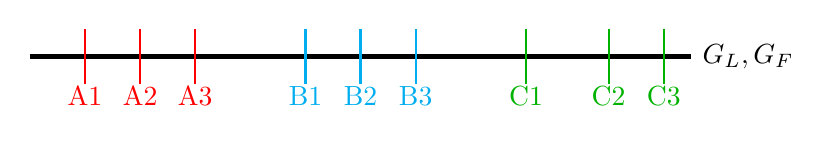
\begin{tikzpicture}[scale=0.7]

\draw[ultra thick] (0,0) -- (12,0) node[right] {$G_L, G_F$};

\draw[thick, red] (1,-0.5) -- (1,0.5) node[below=0.6cm] {A1};
\draw[thick, red] (2,-0.5) -- (2,0.5) node[below=0.6cm] {A2};
\draw[thick, red] (3,-0.5) -- (3,0.5) node[below=0.6cm] {A3};


\draw[thick, cyan] (5,-0.5) -- (5,0.5) node[below=0.6cm] {B1};
\draw[thick, cyan] (6,-0.5) -- (6,0.5) node[below=0.6cm] {B2};
\draw[thick, cyan] (7,-0.5) -- (7,0.5) node[below=0.6cm] {B3};

\draw[thick, green!70!black] (9,-0.5) -- (9,0.5) node[below=0.6cm] {C1};
\draw[thick, green!70!black] (10.5,-0.5) -- (10.5,0.5) node[below=0.6cm] {C2};
\draw[thick, green!70!black] (11.5,-0.5) -- (11.5,0.5) node[below=0.6cm] {C3};
\end{tikzpicture}
\end{center}

\begin{itemize}
\item \textbf{Single-peaked preferences:} each voter has one most-preferred spending level.
\end{itemize}
\vspace{0.1cm}
\footnotesize
\textit{With single-peaked preferences, majority rule selects the median voter’s ideal point.}
\end{frame}


\begin{frame}{Why the Median Outcome Works for $G_F$ but Not for $G_L$}
On that horizontal line, each point is a quantity of the public good. If the good is national ($G_F$), everyone consumes the same quantity once it is chosen, so picking the median voter’s preferred level is efficient. If the good is local ($G_L$), people in different places could consume different quantities, but a centralised vote still forces one single level on everyone, which creates the mismatch.

\begin{center}
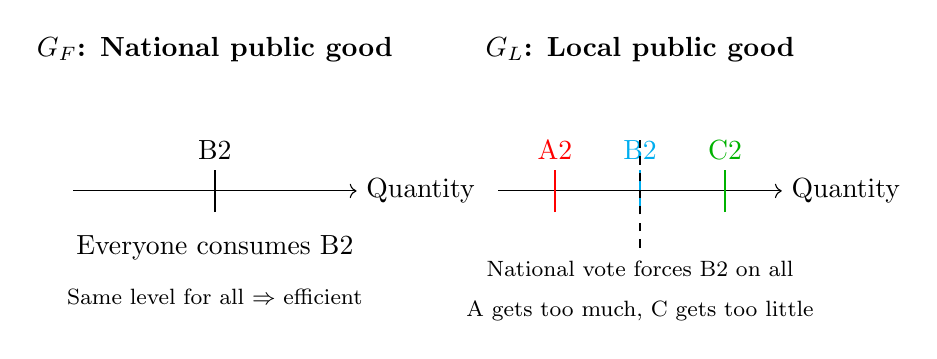
\begin{tikzpicture}[scale=0.9]


\node at (2,4) {\textbf{$G_F$: National public good}};

\draw[->] (0,2) -- (4,2) node[right] {Quantity};
\draw[thick] (2,1.7) -- (2,2.3) node[above] {B2};

\node at (2,1.2) {Everyone consumes B2};

\node at (2,0.5) {\footnotesize Same level for all $\Rightarrow$ efficient};


\node at (8,4) {\textbf{$G_L$: Local public good}};

\draw[->] (6,2) -- (10,2) node[right] {Quantity};


\draw[thick, red] (6.8,1.7) -- (6.8,2.3) node[above] {A2};
\draw[thick, cyan] (8,1.7) -- (8,2.3) node[above] {B2};
\draw[thick, green!70!black] (9.2,1.7) -- (9.2,2.3) node[above] {C2};


\draw[dashed] (8,1.2) -- (8,2.8);
\node at (8,0.9) {\footnotesize National vote forces B2 on all};

\node at (8,0.3) {\footnotesize A gets too much, C gets too little};

\end{tikzpicture}
\end{center}
\end{frame}




\begin{frame}{The Median Voter in a Centralised State}
Applying majority rule to the previous distribution, the national policy is set by the \textbf{median voter’s} ideal point, which in the figure is \textbf{B2}.

\begin{itemize}
\item For $G_F$ (a national public good), this outcome is efficient because everyone consumes the same level.
\item For $G_L$ (a local public good), uniform provision is inefficient:
\begin{itemize}
\item Community A is forced to pay for more than it prefers
\item Community C receives less than it prefers
\end{itemize}
\end{itemize}

\vspace{0.15cm}
\alert{\footnotesize Under federalism: A chooses A2, B chooses B2, and C chooses C2. decentralised choice restores the locally preferred levels for $G_L$.}
\end{frame}


\begin{frame}{The Political Reality: the Madisonian Warning}
Traditional theory assumes a benevolent centre. Public choice emphasises political incentives.

\begin{quote}\small
"For the same reason that the members of the State legislatures will be unlikely to attach themselves sufficiently to national objects, the members of the federal legislature will be likely to attach themselves too much to local objects."\\
- James Madison, \textit{The Federalist}
\end{quote}

The key point is that national representatives are elected from geographic districts, so their incentives are local even when they sit in a national legislature. They will try to direct national spending toward their own constituencies, which means the centre does not automatically behave as a provider of pure national public goods.

\textbf{Implication:} even national institutions can behave like a vehicle for local pork-barrel politics $\rightarrow$ nationally funded projects that deliver concentrated local benefits while spreading the cost across all taxpayers.

\end{frame}

\begin{frame}{The Irish Context: a Centralised Exception?}
Ireland is often described as unusually centralised relative to much of Europe.

\begin{itemize}
\item Health, education, and policing are heavily directed from the centre.
\item \textbf{Local government:} local authorities have fewer powers and smaller budgets than in federal systems (e.g., Germany, Switzerland).
\end{itemize}

\vspace{0.15cm}
\begin{alertblock}{Discussion Question}
Does "one size fits all" national policy create the welfare losses predicted by Oates? Or do small scale and spillovers make centralisation relatively efficient in Ireland?
\end{alertblock}

\vspace{0.15cm}
\footnotesize
In Ireland, local amenities such as parks, planning decisions, and housing density fit Oates’ case for decentralisation because preferences differ and spillovers are limited.
By contrast, hospitals, policing, and major commuter transport generate large inter-county spillovers in a highly integrated labour market, which strengthens the case for central provision.

\end{frame}

\section{II. The Market Solution: Tiebout's "Voting with Feet"}


\begin{frame}{The Challenge: Samuelson's Pessimism}
We have seen that decentralisation can improve welfare for local goods because preferences differ and local governments have better information. Now the question is whether decentralised provision can really be efficient in a market-like sense, given Samuelson’s claim that public goods* cannot be priced properly (they don't generate market prices that reveal demand).
If benefits are non-excludable (everyone benefits whether they pay or not), people have an incentive to free ride, so governments can’t observe true willingness to pay.

\begin{itemize}
\item \textbf{Paul Samuelson (1954):} with public goods, preference revelation fails, so efficient provision is difficult.
\item \textbf{Charles Tiebout (1956):} this pessimism is strongest at the \textit{national} level.
\item The local level has an extra mechanism: \textbf{mobility}.
\end{itemize}


\footnotesize
\textit{Definition: free riding = understating demand because you can benefit even if you don't pay.}\\
* National defence is the classic Irish example: you cannot exclude non-taxpayers from being protected, and one person’s protection does not reduce another’s.
\end{frame}

\begin{frame}{The "Shopping Trip" Analogy}
Tiebout treats local government like a market for \textbf{bundles} of taxes and services.
Instead of buying a product, households choose a place to live.

\begin{enumerate}
\item \textbf{The menu:} jurisdictions offer different bundles (schools, parks, roads) and different tax rates.
\item \textbf{The choice:} people compare bundles and move to the best fit.
\item \textbf{The result (sorting):} similar preferences cluster in the same communities.
\end{enumerate}

\vspace{0.15cm}
\alert{\footnotesize Key implication: "voting with your feet" reveals preferences more credibly than voting alone $\rightarrow$ In the Tiebout model, a household that prefers lower taxes and fewer services moves to a low-tax council area, while a household that values better schools and amenities moves to a higher-tax area that funds them. Because moving involves real costs (housing, job commute, social ties), it is a more credible signal of preferences than a vote, which is costless and often strategic.}
\end{frame}

\begin{frame}{Tiebout's Core Insight (1956)}
Tiebout’s claim is not that local politics is perfect, but that mobility can make it behave \textit{more like} a market.
If people can move, local governments face a form of demand discipline.

\begin{itemize}
\item The local public goods problem can be treated like a \textbf{spatial economy} with location choice.
\item With enough mobility, local provision "need not take a back seat" to private markets.
\item Mechanism: moving is a form of \textbf{revealed preference} because it is costly and consequential.
\end{itemize}

\vspace{0.15cm}
\footnotesize
\textit{Definition: revealed preference = inferring preferences from choices people actually make (here: where they live).}
\end{frame}

\begin{frame}{The Strict Assumptions (the Fine Print)}
For the Tiebout mechanism to deliver an efficient outcome, several assumptions have to hold.
These assumptions are the main reason the model is used as a benchmark rather than a literal description.

\begin{itemize}
\item \textbf{Full mobility:} moving is costless (financially and emotionally).
\item \textbf{Full information:} citizens know the tax/service bundles of each community.
\item \textbf{Many jurisdictions:} enough variety exists to match different preferences.
\item \textbf{No spillovers:} benefits don't cross borders (so the boundary problem disappears).
\item \textbf{Income independent of location:} in the original setup, people can choose location without job constraints ("dividend income").
\end{itemize}

\vspace{0.1cm}
\footnotesize
\textit{So: Tiebout works best when people can move easily and local policies don't affect outsiders.}
\end{frame}

\begin{frame}{The Reality Check: the Fixed Factor}
In practice, mobility is limited, and that limits how far "voting with your feet" can go.
For most households, the binding constraint is not local services but rather where they can earn a living.

\begin{itemize}
\item \textbf{Jobs as the anchor:} employment ties people to a region, so sorting is incomplete.
\item \textbf{The Irish context:}
\begin{itemize}
\item Within Dublin, choices across councils can reflect taxes/services (Tiebout has bite).
\item Moving from Dublin to Leitrim just for lower rates is unlikely if your job is in the IFSC (Tiebout weakens).
\end{itemize}
\end{itemize}

\vspace{0.1cm}
\footnotesize
\textit{Definition: a fixed factor is something that can’t easily move across jurisdictions (here: jobs for most people).}
\end{frame}

\begin{frame}{Evidence: Capitalisation}
One testable implication is that public services should show up in housing markets.
If people value a bundle (e.g., better schools at the same taxes), they bid up property prices in the jurisdictions that offer it.

\begin{itemize}
\item Logic: higher demand to live in community A raises house prices until the price gap reflects the value of the better services.
\item Conclusion: households often pay for local public goods through rent/mortgages rather than through explicit taxes.
\end{itemize}

\vspace{0.15cm}
\footnotesize
\textit{Definition: capitalisation = policy differences being priced into asset values (here: housing).}
\end{frame}

\begin{frame}{The Political Reaction to Tiebout: Cartels}
If mobility creates tax competition, it constrains local politicians’ ability to raise revenue.
Public choice predicts that politicians will try to weaken that constraint. This incentive to escape competition leads jurisdictions to coordinate their policies, which is reflected in the following mechanisms:

\begin{itemize}
\item \textbf{Collusion:} jurisdictions may coordinate to reduce tax competition, like firms forming a cartel.
\item \textbf{Role of the centre:} higher levels can help coordinate harmonisation or use equalisation to blunt competitive pressure.
\item Result: local politicians may willingly surrender autonomy if it reduces the discipline imposed by mobile taxpayers.
\end{itemize}

\vspace{0.1cm}
\footnotesize
\textit{Definition: tax competition = residents can move away from high-tax/low-service bundles, pressuring governments to adjust.}
\end{frame}


\section{III. The Fiscal Toolkit: Grants and the Flypaper Effect}

\begin{frame}[allowframebreaks]{Intergovernmental Grants: the Normative View}
Tiebout gives us a competitive local system, but it only works well when spillovers are small and jurisdictions have similar resources. In practice, some areas are poorer and some policies affect neighbouring regions, so the centre uses intergovernmental grants to change incentives and redistribute fiscal capacity.

Grants are the standard tool for dealing with two problems that decentralisation creates in practice: \textbf{spillovers} and \textbf{unequal fiscal capacity}.
If local decisions affect outsiders, or if some regions cannot fund basic services, the centre can use transfers to change incentives and equalise resources. These two objectives are implemented through different grant designs, which affect local incentives in distinct ways:

\begin{itemize}
\item \textbf{Matching grants:} the centre pays a percentage of the cost of a local project (e.g., highways)
\begin{itemize}
\item \textit{Effect:} lowers the local "price" of the public good, so jurisdictions choose more of it
\item \textit{Use case:} best when the goal is to internalise spillovers
\end{itemize}
\item \textbf{Unconditional / block grants:} a lump-sum transfer with no strings attached
\begin{itemize}
\item \textit{Effect:} raises local income, so councils can spend more \textit{or} cut local taxes
\item \textit{Use case:} best when the goal is redistribution across richer and poorer regions
\end{itemize}
\end{itemize}

\vspace{0.1cm}
\footnotesize
\textit{Definition: fiscal capacity = how much revenue a jurisdiction can raise from its own tax base at reasonable rates.}
\end{frame}

\begin{frame}{The Empirical Anomaly: the Flypaper Effect}
In a simple median-voter model, an unconditional block grant is equivalent to an increase in local private income.
So most of it should show up as \textbf{tax cuts} (more private consumption), not as a large jump in public spending.

\vspace{0.2cm}
\begin{alertblock}{The Reality}
Empirical studies often find that local spending rises by \textbf{25\% to over 200\%} of the grant amount.
\end{alertblock}

\vspace{0.2cm}
\textbf{Flypaper effect:} money transferred from the centre largely "sticks where it lands" in the local government budget.

\vspace{0.1cm}
\footnotesize
\textit{Definition: flypaper effect = grants raise public spending more than an equivalent increase in residents’ private income.}
\end{frame}

\begin{frame}{Flypaper: What Simple Theory Predicts (Hines \& Thaler, 1995)}
\small
The benchmark prediction treats grants as ordinary income: the community allocates the extra resources using its usual spending shares.

\begin{itemize}
\item Treat a lump-sum block grant as \textbf{equivalent to an increase in local private income}
\item Then extra spending on $G$ should match the \textbf{marginal propensity to spend on public goods}
\item Rule of thumb: often described as \textbf{about 5--10 cents per \$1} of extra income (in U.S. state/local contexts)
\item Empirical punchline: many estimates are \textbf{much closer to \$1-for-\$1 spending} than 5--10 cents
\end{itemize}

If people really controlled the budget, a grant should mostly become tax cuts; instead it turns into spending, which suggests political or bureaucratic factors change how the money is used.

\vspace{0.15cm}
\footnotesize
\textit{Intuition: the same budget constraint seems to produce different choices depending on whether money arrives as income or as a grant.}
\end{frame}

\begin{frame}{Public Choice Explanations for the Flypaper Effect}
If grants systematically increase spending more than standard theory predicts, the natural question is \textbf{where the decision process differs}.
Public choice points to politics and bureaucracy rather than preferences alone. These mechanisms change how voters perceive costs and how officials allocate funds, as reflected in the following explanations:


\begin{enumerate}
\item \textbf{Fiscal illusion (Puviani, Italian public finance scholar from the late 19th century):} voters do not fully perceive that grant money is ultimately their money, so politicians can spend it with less backlash than raising visible local taxes
\item \textbf{Bureaucratic power (Niskanen, public choice economist who proposed the budget-maximising bureaucrat model):} bureaucrats maximise budgets and exploit information advantages to steer grant resources into departmental spending rather than tax cuts
\end{enumerate}

\vspace{0.1cm}
\footnotesize
\textit{Definition: fiscal illusion = voters underestimate the true cost of public spending when it is financed indirectly or opaquely.}
\end{frame}


\section{IV. Politics Without Romance: Federalism's Pathologies}

\begin{frame}{Why Government Gets "Too Large": Universalism}
When the centre funds local projects, \textbf{benefits are concentrated} in one district while \textbf{costs are spread} across national taxpayers.
That wedge changes incentives: representatives can claim credit locally while exporting part of the bill. These spending patterns are reinforced inside legislatures, where representatives have incentives to support each other’s locally targeted projects.


\begin{itemize}
\item \textbf{Logrolling (Tullock’s roads):} representatives trade votes to fund each other’s local projects.
\item \textbf{Universalism norm:} legislatures often move from "some districts win" to "everyone gets something" when the centre supplies local goods.
\item \textbf{Result:} packages of local projects get approved centrally that would have been rejected if each locality paid the full marginal cost itself.
\end{itemize}

\vspace{0.1cm}
\footnotesize
\textit{Definition: logrolling = vote trading across legislators to form a majority for each other’s projects.}
\end{frame}

\begin{frame}{"Too Large" and "Too Small" Simultaneously}
Geographic representation can push spending in two directions at once.
It can expand localised projects while leaving too little fiscal space for genuine national public goods. This creates a composition effect within a fixed budget, which is reflected in the following incentives and outcomes:

\begin{itemize}
\item Politicians maximise votes by supplying both national and local goods, but local projects deliver clearer, district-level credit.
\item \textbf{Crowding out:} as more resources are steered to local projects, national public goods are squeezed within the same budget constraint.
\end{itemize}

\vspace{0.15cm}
\alert{\footnotesize With grants and geographic representation: "too much" local spending and "too little" national spending can coexist.}
\end{frame}

\begin{frame}{A Case Study: the European Union}
The EU is a useful illustration because it combines geographic representation with a tight overall budget.
When redistribution dominates, EU-wide public goods become residual claimants. This institutional setup produces the same incentives we just discussed, which can be observed in the EU budget composition:


\begin{itemize}
\item The EU Council is based on national representation and operates under a small budget relative to GDP.
\item \textbf{Composition:} historically, a large share of spending has been redistributional (e.g., agricultural subsidies).
\item \textbf{Opportunity cost:} if most funds are absorbed by national returns, less remains for EU-wide public goods (foreign policy, defence, cross-border infrastructure).
\end{itemize}

\end{frame}

\begin{frame}{The Threat of Centralisation: Popitz's Law}
Popitz’s* Law is a claim about drift: over time, fiscal authority tends to move toward the centre.
In Mueller’s telling, the key mechanism is political incentives rather than administrative efficiency.

\begin{itemize}
\item \textbf{Germany example:} subnational shares of tax revenue fell sharply over the postwar period.
\item \textbf{Mechanism:} local politicians can be willing accomplices if centralisation reduces tax competition and softens local fiscal discipline.
\end{itemize}

\vspace{0.1cm}
\textbf{Can it be resisted?} Switzerland is often used as a contrast case: referenda and direct democracy can make tax and spending expansions easier to block.


\vspace{0.1cm}
\footnotesize
\textit{Definition: centralisation drift = gradual transfer of taxing/spending authority upward through harmonisation, mandates, and transfers.}
* Popitz was a German public finance official and scholar active in the early 20th century. He served in the Prussian Ministry of Finance and later became Reich Finance Minister in the 1930s, so his work came from practical experience with intergovernmental fiscal relations.
\end{frame}


\section{V. Institutional Guardrails: Market-Preserving Federalism}

\begin{frame}{Popitz's Law: Not Just a Power Grab}
\small
Popitz’s Law is often presented as a drift toward the centre, but Mueller’s account stresses \textbf{political incentives}.
Centralisation can be attractive to local politicians if it reduces competitive pressure and makes spending less costly at the margin.

\begin{itemize}
\item Mechanism is \textbf{political economy}:
\begin{itemize}
\item Subnational politicians can be \textbf{willing accomplices} because they dislike tax competition
\item The centre can help \textbf{organise a cartel} that compresses regional tax differences
\end{itemize}
\item Implication: centralisation can \textbf{increase the scale of government}
\item Contrast case: Switzerland, where \textbf{referenda and direct democracy} can block tax and spending expansions
\end{itemize}

\vspace{0.1cm}
\footnotesize
\textit{Definition: cartel (in this context) = coordinated behaviour across jurisdictions to reduce fiscal competition (e.g., harmonising rates).}
\end{frame}

\begin{frame}{Market-Preserving Federalism (Weingast, 1995)}
Weingast* starts from a dilemma: a state strong enough to protect property rights is also strong enough to confiscate wealth.
The question is which institutions make restraint credible.

\begin{enumerate}
\item \textbf{Subnational autonomy:} key regulatory and economic authority resides with lower tiers, not only at the centre
\item \textbf{Common market:} the centre polices internal trade and prevents barriers between regions
\item \textbf{Hard budget constraints:} local governments cannot print money and cannot expect systematic bailouts
\end{enumerate}

\vspace{0.1cm}
\alert{\footnotesize Result: governments face competitive and fiscal constraints that make predation more costly when capital and taxpayers can move.} \\
\footnotesize
* Barry R. Weingast is an American political economist (Stanford) associated with the “new institutional economics”. His 1995 paper on market-preserving federalism tries to explain why some federal systems (notably the U.S. in the 19th century and post-reform China at the provincial level) supported economic growth while others did not.
\end{frame}

\begin{frame}[allowframebreaks]{Hard vs. Soft Budget Constraints}
Weingast’s market-preserving federalism addresses the credible commitment problem by making predation costly: subnational governments control economic policy, capital and labour can move, and a national common market prevents protectionist barriers. Hard budget constraints force local fiscal discipline, so jurisdictions compete to protect property rights and attract investment.
The credibility of decentralisation depends on whether local governments face the full consequences of their choices.
If failure is routinely rescued by the centre, local incentives change. The following conditions define the institutional features required for federalism to support market activity:

\begin{itemize}
\item \textbf{Soft budget constraint:} if local deficits are routinely bailed out by the centre, local politicians can overspend or under-tax because part of the cost is shifted to national taxpayers (moral hazard).
\item \textbf{Hard budget constraint:} if bailouts are not expected, deficits must be covered locally through taxes, spending cuts, or borrowing at market rates, which increases accountability to local voters and creditors.
\end{itemize}

\vspace{0.1cm}
\footnotesize
\textit{Implication: credible no-bailout rules make interjurisdictional competition and Tiebout-style discipline more effective.}


\vspace{0.1cm}
\footnotesize
\textit{Definition: soft budget constraint = expectation of rescue that weakens incentives to balance budgets.}
\end{frame}

\begin{frame}{Laboratory Federalism}
Decentralisation can also create a learning advantage over time.
When policy is uncertain, multiple jurisdictions can try different approaches and generate evidence about what works.

\begin{itemize}
\item \textbf{States as laboratories:} subnational units experiment with policy designs under real constraints
\item \textbf{Learning and diffusion:} successful policies can be copied by other regions or scaled up nationally
\item \textbf{Risk mitigation:} policy failure is contained rather than imposed nationwide
\end{itemize}

\vspace{0.1cm}
\footnotesize
\textit{Definition: diffusion = adoption of a policy by other jurisdictions after observing outcomes elsewhere.}
\end{frame}


\section{VI. Evidence and Context: Corruption and the Global Picture}

\begin{frame}[allowframebreaks]{Does Decentralisation Increase Corruption?}
Decentralisation can improve accountability, but it can also create a problem of \textbf{uncoordinated rent-seeking}.
If multiple layers of government can extract from the same firms, each layer ignores the damage its extraction imposes on the others. This mechanism can be understood by viewing taxation authority as a shared resource, which leads to the following commons-type incentives:

\begin{itemize}
\item \textbf{"Overgrazed" tax base:} local, regional, and national actors can all try to tax or extract bribes from the same business, creating excessive total extraction.
\item \textbf{Tragedy of the commons logic:} each layer takes what it can, ignoring that it reduces the overall tax base and pushes activity into informality.
\item Contrast: a single central extractor may internalise the long-run value of keeping the "goose" productive, even if governance is worse in other respects.
\end{itemize}

\vspace{0.1cm}
\footnotesize
\textit{Definition: rent-seeking = using political power to obtain transfers (rents) rather than creating new economic value.}
\end{frame}

\begin{frame}[allowframebreaks]{Evidence: Decentralisation and Corruption (Fan, Lin \& Treisman, 2009)}
\small
The empirical question is \textbf{which type} of decentralisation is changing.
Different institutional margins imply different accountability and oversight channels.

\begin{itemize}
\item Question: does decentralisation reduce corruption through accountability, or raise it through weaker oversight
\item Key distinction: decentralisation is multidimensional
\begin{itemize}
\item \textit{Fiscal decentralisation:} subnational spending/revenue autonomy
\item \textit{Political/administrative decentralisation:} local elections, local control of officials
\end{itemize}
\item Evidence approach: cross-country regressions linking decentralisation measures to corruption indices
\item Main takeaway: the relationship is \textbf{not one-directional} and depends on institutional context and what is decentralised
\item Link back to theory: if oversight is weak and multiple layers extract from the same base, decentralisation can intensify rent-seeking
\end{itemize}

\vspace{0.1cm}
\footnotesize
\textit{Definition: fiscal decentralisation = subnational control over revenues/spending rather than only delegated administration.}
\end{frame}

\begin{frame}{Why the Evidence is Mixed}
\small
A mixed literature is not surprising because both theory and measurement point to heterogeneity.
The same reform label can mean different institutional changes in different countries.

\begin{itemize}
\item \textbf{Endogeneity:} countries decentralise for political reasons that may also correlate with corruption
\item \textbf{Measurement:} decentralisation indicators are imperfect and not fully comparable across systems
\item \textbf{Heterogeneity:} effects vary with institutional guardrails
\begin{itemize}
\item Audit capacity and courts
\item Local media and civic monitoring
\item Party systems and electoral competition
\item Hard vs. soft budget constraints
\end{itemize}
\item Empirical implication: expect different signs across settings, then ask which institutions are doing the work in a given case
\end{itemize}

\vspace{0.1cm}
\footnotesize
\textit{Definition: endogeneity = decentralisation is not randomly assigned, so simple comparisons can mix cause and selection.}
\end{frame}

\begin{frame}{Service Failure, Exit, and Corruption Dynamics}
When local services deteriorate, decentralisation does not automatically produce stronger accountability.
If the groups with the greatest monitoring capacity leave first, political oversight can collapse.

\begin{enumerate}
\item \textbf{Initial failure:} mismanagement or corruption lowers the quality of local public services
\item \textbf{Selective exit:} higher-income households move to private alternatives (schools, healthcare)
\item \textbf{Weaker voice:} remaining users have less time, information, and political influence to monitor officials
\item \textbf{Entrenchment:} lower scrutiny reduces the cost of rent-seeking, so performance declines further
\end{enumerate}

\vspace{0.15cm}
\alert{\footnotesize Policy intuition: broad-based local taxation keeps more residents financially and politically invested in monitoring local government.}
\end{frame}



\begin{frame}{Empirical Outcomes: Does it Work?}
When institutional guardrails are present (local taxation, hard budget constraints, credible oversight), decentralisation can improve outcomes.
Two standard examples in this literature illustrate the mechanism: closer matching of spending to local needs and stronger discipline from local accountability.

\begin{itemize}
\item \textbf{Swiss cantons (Barankay \& Lockwood, 2007):}
\begin{itemize}
\item decentralisation is associated with higher educational attainment
\item improvements occur without adverse equity effects in their setting
\end{itemize}
\item \textbf{Bolivia (Faguet, 2004):}
\begin{itemize}
\item decentralisation shifted investment toward human capital and basic services (education, water)
\item spending patterns aligned more closely with measured local needs than under centralised allocation
\end{itemize}
\end{itemize}

\vspace{0.1cm}
\footnotesize
\textit{Definition: accountability channel = local officials face stronger incentives when voters can better observe performance and fiscal choices.}
\end{frame}

\section{Conclusion}

\begin{frame}{Summary: federalism without romance}
\begin{enumerate}
\item \textbf{Assignment logic:} decentralisation can raise welfare for \textit{local} goods when preferences and costs differ across places (Oates), and it can use local knowledge that the centre cannot aggregate (Hayek)
\item \textbf{Mobility discipline:} when people and capital can move, jurisdictions face competitive pressure that can reveal preferences and constrain taxation (Tiebout)
\item \textbf{Political economy:} intergovernmental grants, logrolling, and universalism can expand localised spending while crowding out national public goods, and centralisation drift can emerge through cartel-like harmonisation (Mueller/Popitz)
\item \textbf{Guardrails and risks:} decentralisation performs better with hard budget constraints, local taxation, and credible oversight; without them, soft budgets and uncoordinated rent-seeking can weaken accountability
\end{enumerate}
\end{frame}


\section*{The Irish Context: Federalism in a Centralised State}

\begin{frame}{The Irish Anomaly: Extreme Centralization}
\textbf{A 2023 \href{https://rm.coe.int/monitoring-of-the-application-of-the-european-charter-of-local-self-go/1680acd809}{Council of Europe Report on Ireland} found:}
\begin{itemize}
\item Ireland remains one of the most centralised countries in Europe.
\item It is compliant with only \href{https://ailg.ie/european-body-issues-damning-report-on-irish-local-government/}{8 out of 20} principles of the European Charter of Local Self-Government.
\item \textbf{Financial Autonomy:} local authorities have highly limited "own-source" financial resources that can be used at their discretion.
\item \textbf{Subsidiarity Failure:} the state is far from complying with the principle of subsidiarity, meaning decisions are taken far away from the local citizen.
\end{itemize}
\vspace{0.3cm}
\alert{Question: Does this centralization create the welfare losses predicted by Oates?}
\end{frame}

\begin{frame}{How Local Government is Funded}
Since they lack broad tax-raising powers, Irish local councils rely heavily on:
\begin{enumerate}
\item \textbf{Commercial Rates:} taxes levied on business properties.
\item \textbf{Central Government Grants:} specific/earmarked grants (e.g., for roads or housing) which strictly limit local policy discretion.
\item \textbf{Local Property Tax (LPT):} introduced in 2013, an annual self-assessed tax based on residential market values.
\end{enumerate}
\vspace{0.3cm}
\textit{Because central grants are heavily earmarked, local councils often experience the Flypaper Effect without the freedom to innovate.}
\end{frame}

\begin{frame}{The Local Property Tax (LPT) as a Tiebout Mechanism?}
The LPT introduced an important element of decentralisation:
\begin{itemize}
\item \textbf{The Local Adjustment Factor:} since 2015, local authorities can vary the base LPT via a Local Adjustment Factor (±15\%). From 2026 onward, they can vary upwards by up to +25\%, and downwards by up to −15\%.
\item \textbf{The Tiebout Logic:} this allows a council (e.g., Fingal) to lower taxes to attract residents, or raise taxes to fund better local services.
\end{itemize}

\alert{The Constraint: the Equalisation Fund}
\begin{itemize}
\item 20\% of the LPT collected in wealthier areas is diverted to an "Equalisation Fund" to subsidize poorer councils (like Longford or Leitrim).
\item This redistributive mechanism weakens the pure "benefit tax" link that Tiebout and Weingast argue is necessary for hard budget constraints.
\end{itemize}
\end{frame}

\begin{frame}{Oates vs. Irish Geography: Spillovers}
Is centralization actually efficient for Ireland?

\textbf{The Geography of Spillovers:}
\begin{itemize}
\item Under Oates' Decentralisation Theorem, local goods should be locally funded.
\item However, Ireland is geographically small with highly integrated labour markets.
\item If Kildare funds a new road, commuters from Meath and Dublin use it (a massive positive externality / boundary problem).
\end{itemize}
\alert{Conclusion:} the small scale of the country and the high potential for inter-county spillovers provide a strong traditional economic justification for centralizing health, transport, and police, despite the Council of Europe's political critiques.
\end{frame}


\section*{Further Readings}

\begin{frame}[allowframebreaks]{Further Readings: Foundational Theory of Fiscal Federalism}
\footnotesize
\begin{itemize}
\item Mueller, Dennis C. (2003) - \textit{Public Choice III}, Chapter 10.\\
\textit{Textbook roadmap: assignment problem, decentralisation theorem, Tiebout, grants, and public choice frictions.}

\item Oates, Wallace E. (1972) - \textit{Fiscal Federalism}.\\
\textit{Classic statement of the decentralisation theorem and spillovers/assignment logic.}

\item Hayek, F. A. (1945) - "The Use of Knowledge in Society."\\
\textit{Why local knowledge is hard to aggregate; centralised decisions can misallocate resources.}

\item Samuelson, Paul A. (1954) - "The Pure Theory of Public Expenditure."\\
\textit{Public goods problem: efficient provision needs preference information governments usually can't elicit.}

\item Tiebout, Charles M. (1956) - "A Pure Theory of Local Expenditures."\\
\textit{Sorting via mobility: local bundles of taxes and services as a preference-revelation mechanism.}

\item Boex, Jamie; Williamson, Tim; Yilmaz, Serdar (2022) - \textit{Fiscal Decentralisation, Local Public Sector Finance, and Intergovernmental Fiscal Relations: A Primer} (World Bank).\\
\textit{Practical primer on assignment, transfers, and design trade-offs in real intergovernmental systems.}\\
\href{https://documents1.worldbank.org/curated/en/099225502022316135/pdf/P1754490fe142c0db095050e3808607c8ff.pdf}{(PDF)}
\end{itemize}
\end{frame}


\begin{frame}[allowframebreaks]{Further Readings: Public Choice Pathologies \& Guardrails}
\footnotesize
\begin{itemize}
\item Brennan, Geoffrey \& Buchanan, James M. (1980) - \textit{The Power to Tax}.\\
\textit{Leviathan government: decentralisation and fiscal competition as constraints on revenue-maximising states.}

\item Weingast, Barry R. (1995) - "The Economic Role of Political Institutions: Market-Preserving Federalism and Economic Development."\\
\textit{Federal structures as credible limits on predation; conditions under which markets are protected.}

\item Madison, James (1787--1788) - \textit{The Federalist Papers} (e.g., No. 10 and No. 51).\\
\textit{Faction and institutional incentives: why political actors centralise power, and why constraints are needed.}

\item Hines, James R. \& Thaler, Richard H. (1995) - "The Flypaper Effect."\\
\textit{Grants often raise public spending more than equivalent increases in private income.}

\item Rodden, Jonathan (2006) - \textit{Hamilton's Paradox: The Promise and Peril of Fiscal Federalism}.\\
\textit{Soft budget constraints, bailouts, and why some federations generate fiscal discipline while others don't.}\\
\href{https://www.cambridge.org/core/books/hamiltons-paradox/165995D3EAB511F97EC2A65246F985FF}{(Cambridge Core)}

\item Puviani, Amilcare (1897, 1903) - \textit{Theory of Fiscal Illusion} (original Italian works).\\
\textit{Early statement of fiscal illusion; cited in modern flypaper discussions.}

\item Niskanen, William A. (1971) - \textit{Bureaucracy and Representative Government}.\\
\textit{Budget-maximising bureaucrat model used as a flypaper mechanism.}

\item Courant, Paul N.; Gramlich, Edward M.; Rubinfeld, Daniel L. (1979) - "The Stimulative Effects of Intergovernmental Grants."\\
\textit{Classic empirical work in the flypaper literature.}

\item Chernick, Howard (1979) - "An Economic Model of the Distribution of Project Grants."\\
\textit{Why "earmarked" grants can behave like matching grants in practice.}


\end{itemize}
\end{frame}


\begin{frame}[allowframebreaks]{Further Readings: Empirical Evidence \& Centralisation Pressures}
\footnotesize
\begin{itemize}
\item Barankay, Iwan \& Lockwood, Ben (2007) - "Decentralisation and the Productive Efficiency of Government: Evidence from Swiss Cantons."\\
\textit{Empirical evidence on decentralisation and efficiency in spending (Swiss cantons).}

\item Faguet, Jean-Paul (2004) - "Does Decentralisation Increase Government Responsiveness to Local Needs? Evidence from Bolivia."\\
\textit{Decentralisation linked to shifts in investment towards locally valued services (Bolivia).}

\item Gurgur, Tugrul (2016) - "Voice, Exit and Local Capture in a Federation."\\
\textit{Exit/voice can discipline governments, but can also interact with capture and uneven regional capacity.}

\item Popitz, Johannes (1927) - \textit{Der künftige Finanzausgleich zwischen Reich, Ländern und Gemeinden} (Popitz's Law).\\
\textit{Centralisation drift: higher levels tend to absorb fiscal capacity over time via transfers and mandates.}

\item Treisman, Daniel (2007) - \textit{The Architecture of Government: Rethinking Political Decentralisation}.\\
\textit{Sceptical synthesis: why theoretical claims are often underspecified and empirical findings are mixed.}\\
\href{https://www.cambridge.org/core/books/architecture-of-government/D9B2FD6886A1DF8E911A1ABAF5C1F50D}{(Cambridge Core)}

\item Nakatani, Ryota (2025) - "Preventing Fiscal Crises under Decentralisation: Intergovernmental Policies and Institutions" (IMF Working Paper 25/87).\\
\textit{Tools to reduce subnational crisis risk: borrowing rules, oversight, and the design of transfers.}\\
\href{https://www.imf.org/-/media/Files/Publications/WP/2025/English/wpiea2025087-print-pdf.ashx}{(PDF)}
\item Blankart, Charles B. (2000) - work on Popitz's Law in Germany (as cited in Mueller).\\
\textit{German centralisation mechanism via subnational cartel behaviour.}

\item Grossman, Philip J. \& West, Edwin G. (1994) - centralisation and equalisation in Canada (as cited in Mueller).\\
\textit{Parallel "cartel + centre" story for Canada.}

\item Vaubel, Roland (1994; 1996) - referenda and deterrence of centralisation (as cited in Mueller).\\
\textit{Cross-national evidence linking referenda to resistance against centralisation drift.}

\item Frey, Bruno S. (1994) - discussion of the Swiss case (as cited in Mueller).\\
\textit{Institutions behind Switzerland's resistance to Popitz-type drift.}

\item Goodman (1996) - EU budget category source for Mueller's Table 10.1.\\
\textit{Primary source behind the 1985/1995 redistribution shares.}

\item Inman, Robert P. \& Rubinfeld, Daniel L. (1997) - survey of fiscal federalism / public choice literature (as cited in Mueller).\\
\textit{High-level map of theory, institutions, and evidence.}

\end{itemize}
\end{frame}

\section*{Cultural Resources}

\begin{frame}{TV Series: Local Government in Action}
\textbf{Bureaucracy, Spillovers, and Local Politics:}
\begin{itemize}
\item \textbf{Show Me a Hero (HBO, 2015):} a brilliant miniseries on local government navigating federal mandates, racial segregation, and housing in Yonkers, NY. A perfect illustration of the "boundary problem" and local political pressure.
\item \textbf{The Wire (Season 3-5):} explores the decline of the American city through the lens of local politics. It shows the tension between the Mayor's office, the state governor, and the crushing reality of unfunded mandates.
\item \textbf{Parks and Recreation (2009-2015):} a comedic but highly accurate look at the daily operations, budget battles, and citizen interactions within a municipal department.
\end{itemize}
\end{frame}

\begin{frame}{Films \& Documentaries}
\begin{itemize}
\item \textbf{Chinatown (1974):} a classic neo-noir that is fundamentally about the economics of public goods - specifically, the California Water Wars and the extraction of resources from one jurisdiction to feed another.
\item \textbf{City Hall (2020):} Frederick Wiseman’s documentary exploring the government of Boston. It showcases the vast array of localized services a city provides, from eviction prevention to economic advancement task forces.
\item \textbf{Milk (2008):} chronicles the election of Harvey Milk to the San Francisco Board of Supervisors, demonstrating how local government serves as the entry point for marginalized groups to gain political voice.
\end{itemize}
\end{frame}


\section*{Appendices}

\begin{frame}{Appendix A: Oates' Decentralisation Theorem (1/2)}
\textbf{The Setup:}
Assume two jurisdictions (1 and 2) of equal size. They face a constant marginal cost ($MC$) of providing a public good.

\begin{itemize}
\item \textbf{Demand:} jurisdiction 1 has a high demand ($D_1$) for the public good. Jurisdiction 2 has a low demand ($D_2$).
\item \textbf{Decentralised Outcome:} local governments set $MB = MC$. 
\begin{itemize}
\item Jurisdiction 1 consumes $Q_1$.
\item Jurisdiction 2 consumes $Q_2$.
\end{itemize}
\item \textbf{Centralised Outcome:} the national government provides a uniform level of the public good across both regions. It compromises and provides $Q_c$ (where $Q_2 < Q_c < Q_1$).
\end{itemize}
\end{frame}

\begin{frame}{Appendix A: The Welfare Loss of Centralization (2/2)}


\textbf{The Geometric Proof of Welfare Loss:}
under the centralised uniform provision ($Q_c$):
\begin{enumerate}
\item \textbf{Jurisdiction 1 (High Demand):} receives $Q_c$ but actually wants $Q_1$. The lost surplus from under-provision is the triangle formed between $D_1$ and the $MC$ curve, between $Q_c$ and $Q_1$.
\item \textbf{Jurisdiction 2 (Low Demand):} receives $Q_c$ but only wants $Q_2$. They are forced to pay for units they value less than the cost. The deadweight loss of over-provision is the triangle formed between the $MC$ curve and $D_2$, between $Q_2$ and $Q_c$.
\end{enumerate}

\alert{Conclusion:} the total welfare loss of centralization is the sum of these two deadweight loss triangles. Decentralisation eliminates this loss by allowing $Q_1$ and $Q_2$.
\end{frame}

\begin{frame}{Appendix B: Microeconomics of the Flypaper Effect (1/2)}
\textbf{The Standard Income Effect Model:}
imagine a community as a single consumer (the Median Voter) allocating resources between \textbf{Private Goods ($X$)} and \textbf{Local Public Goods ($G$)}.

\begin{itemize}
\item \textbf{Initial Budget Constraint:} the community's income $Y$ dictates the budget line: $Y = P_xX + P_gG$.
\item \textbf{Lump-Sum Grant:} the central government gives an unconditional grant of size $Z$.
\item \textbf{The Shift:} the budget constraint shifts outward parallel to the original line. The new budget is $(Y + Z) = P_xX + P_gG$.
\end{itemize}
\end{frame}

\begin{frame}{Appendix B: The Theoretical Anomaly (2/2)}


\textbf{What Theory Predicts vs. What Happens:}
\begin{itemize}
\item \textbf{The Microeconomic Prediction:} because the grant $Z$ acts exactly like an increase in community income $Y$, the Median Voter should allocate the grant according to their normal marginal propensity to consume. If they normally spend 10\% of their income on public goods and 90\% on private goods, they should spend 10\% of the grant on $G$ and use the other 90\% to cut local taxes (increasing $X$).
\item \textbf{The Flypaper Reality:} empirical data shows that almost 100\% of the grant $Z$ is spent on $G$, and almost none is used to cut local taxes. 
\end{itemize}

\alert{Conclusion:} the Flypaper Effect violates standard consumer choice theory, forcing us to use Public Choice models (Fiscal Illusion or Bureaucratic Slack) to explain why the money "sticks" where it hits.
\end{frame}

\end{document}